\subsection{Twitter}
\begin{frame}[c]\frametitle{Twitter}

\begin{block}{Qué es Twitter}
    \begin{itemize}
        \item Red social creada en el 2006
        \item Usuarios variados
        \item Tuits de hasta 140 caracteres{\footnote{Recientemente han aumentado el límite a 280 caracteres.}}
        \item \alert{Todos los tuits son públicos}
    \end{itemize}
\end{block}

\begin{block}{¿Por qué Twitter?}
    \begin{itemize}
        \item API pública para obtener tuits de cualquier persona
        \item Tópicos muy variados (gran diferencia con portales de noticias, por ejemplo)
        \item Reproducibilidad
    \end{itemize}
    
\end{block}


\end{frame}

\subsection{Búsquedas geolocalizadas}

\begin{frame}[c]\frametitle{Búsquedas geolocalizadas}


\begin{figure}
    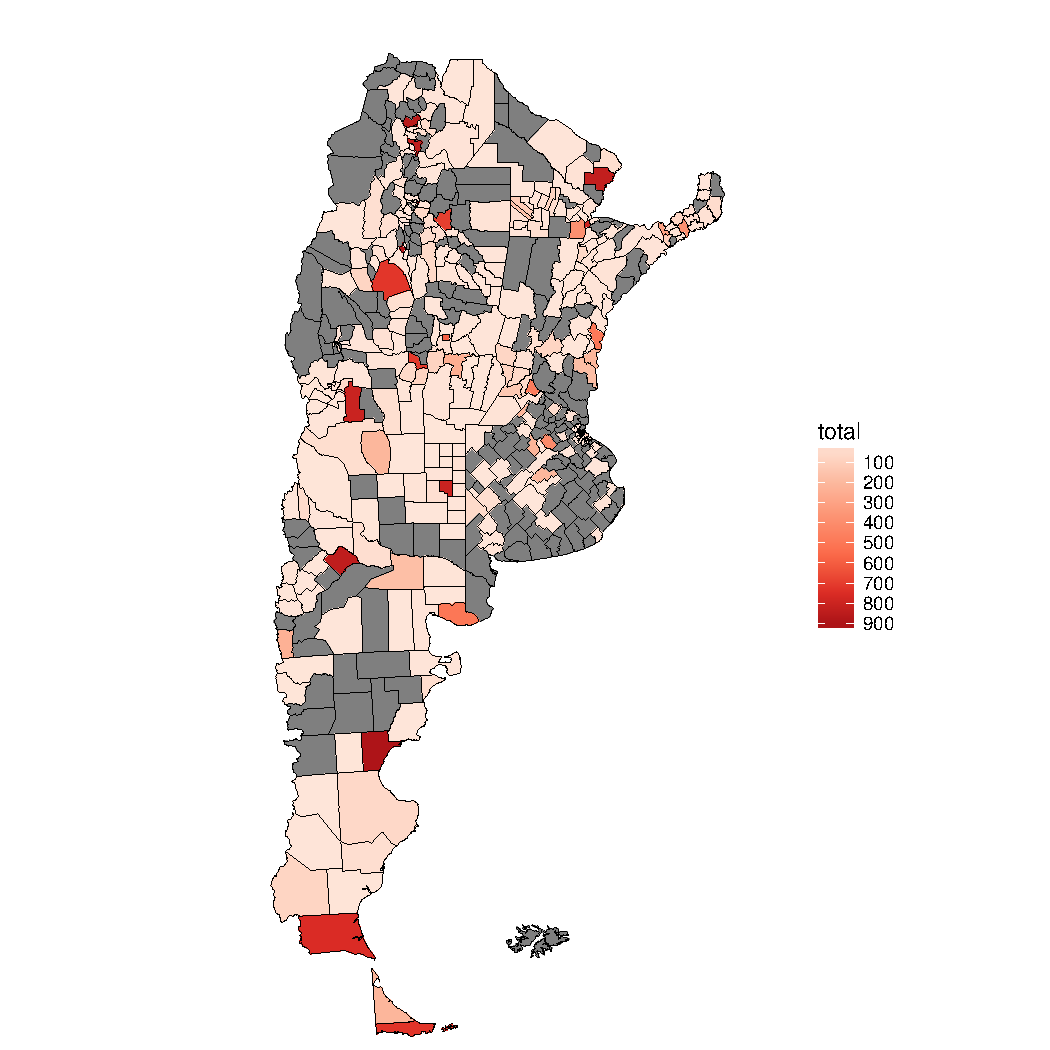
\includegraphics[height=0.5\textheight]{../src/images/mapadepartamentos.pdf}
    % \caption{} 
    \label{fig:mapaDepartamentos}
\end{figure}

% \begin{columns}
%     \begin{column}{0.30\textwidth}
%         \begin{figure}
%             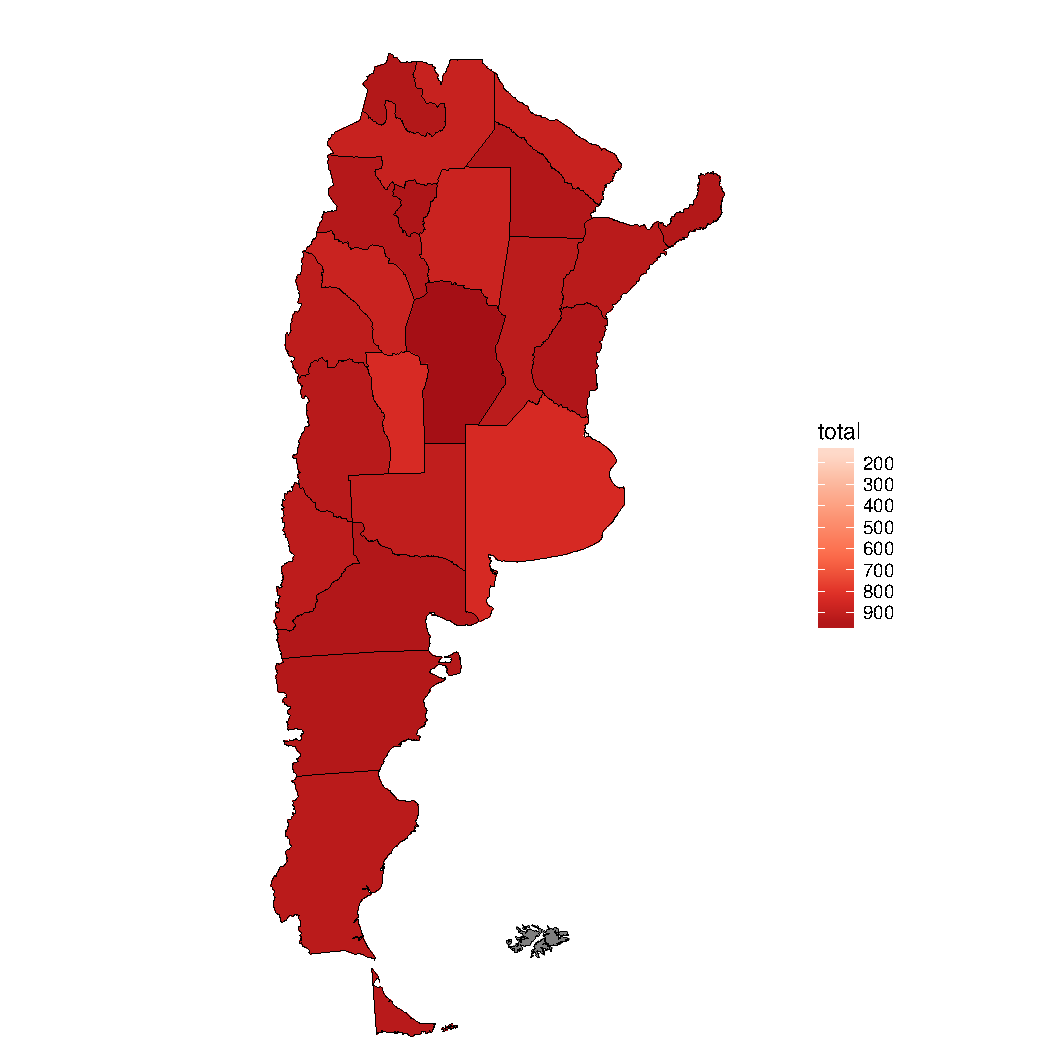
\includegraphics[width=\linewidth]{../src/images/mapaprovincias.pdf}
%             % \caption{} 
%             \label{fig:mapaProvincias}
%         \end{figure}
%     \end{column}

%     \begin{column}{0.30\textwidth}
%         \begin{figure}
%             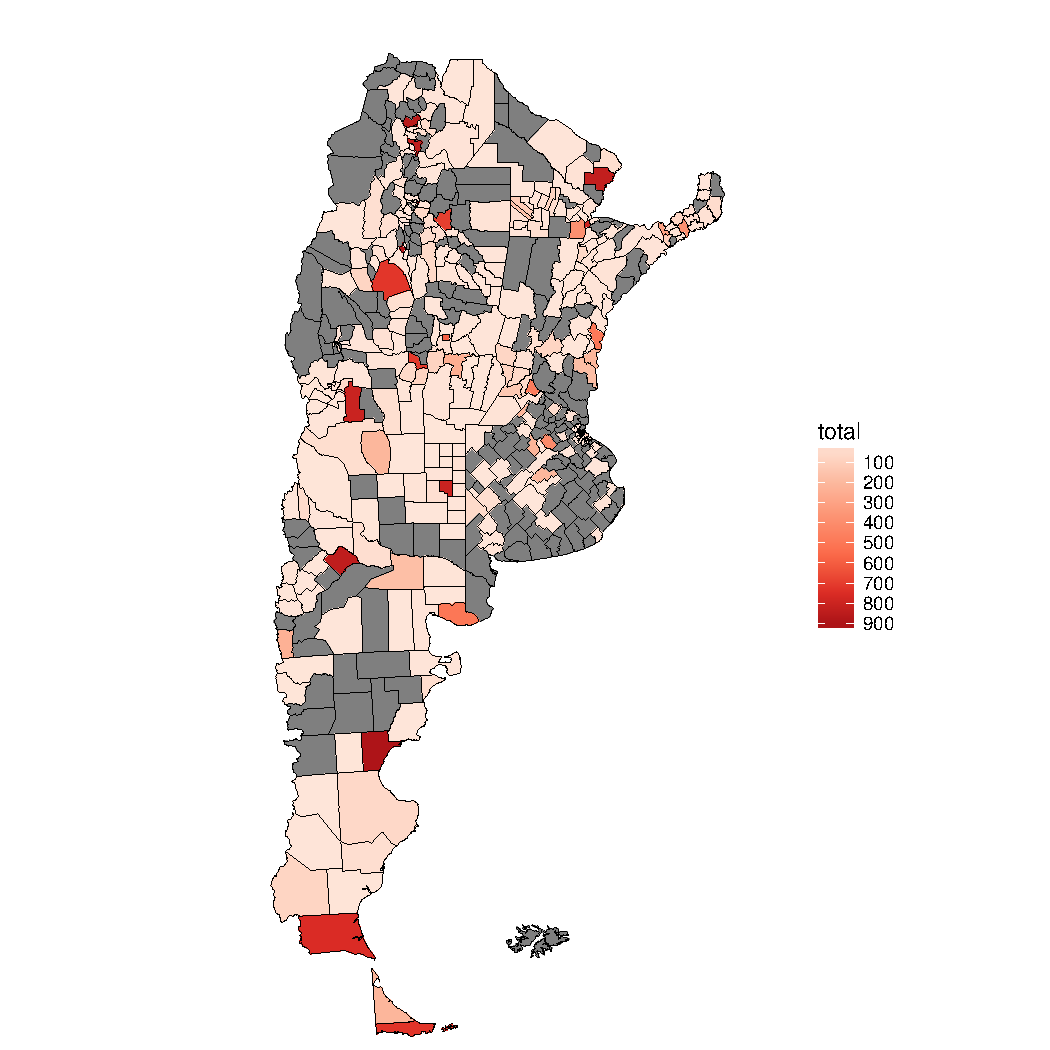
\includegraphics[width=\linewidth]{../src/images/mapadepartamentos.pdf}
%             % \caption{} 
%             \label{fig:mapaDepartamentos}
%         \end{figure}
%     \end{column}

%     \begin{column}{0.30\textwidth}
%         \begin{figure}
%             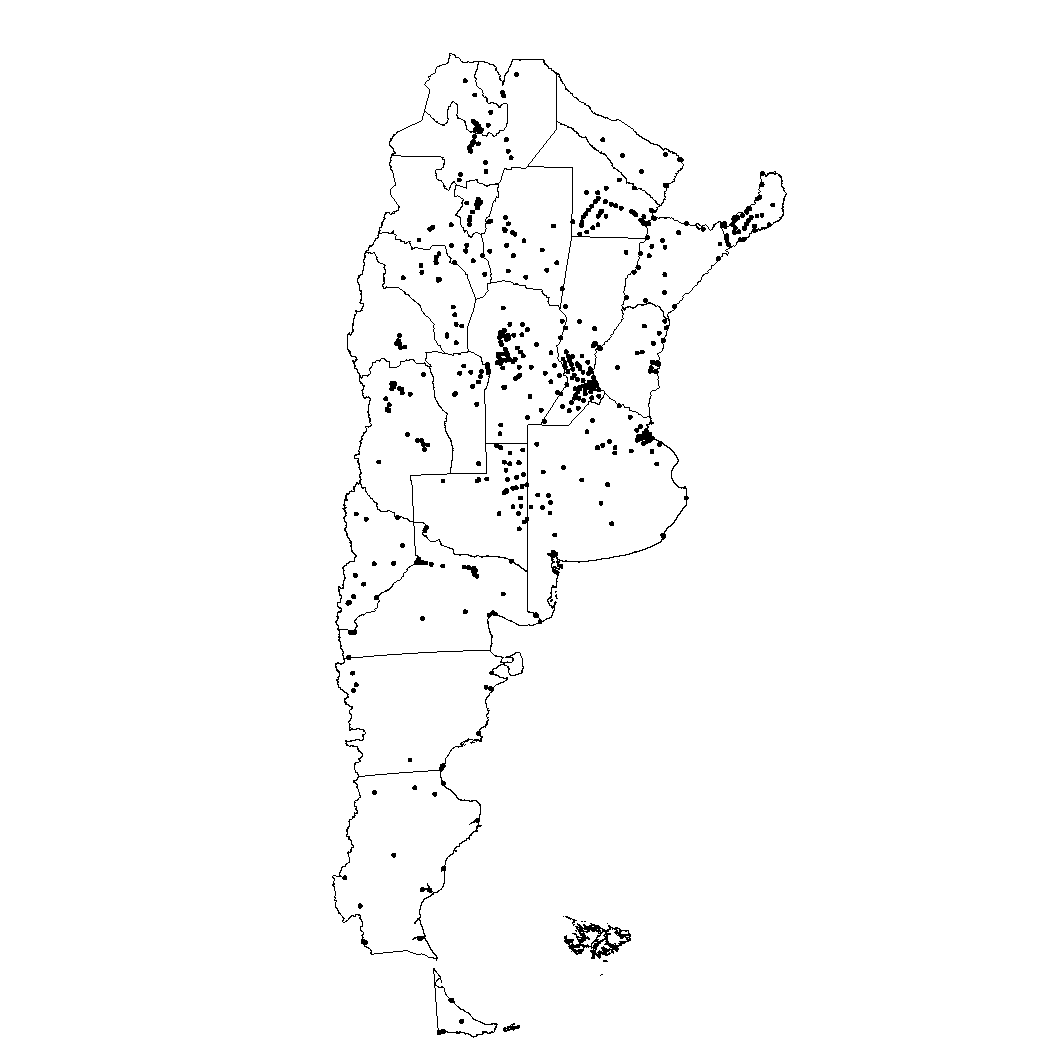
\includegraphics[width=\linewidth]{../src/images/mapaprovinciasConPuntos.pdf}
%             % \caption{} 
%             \label{fig:mapaPuntos}
%         \end{figure}
%     \end{column}
% \end{columns}

\begin{itemize}
    \item Se realizaron búsquedas en todos los departamentos de las provincias argentinas.
    \item Nos quedamos con los usuarios que ingresaron en el campo \textit{location} al menos uno de los nombres de las ciudades de la provincia. 

\end{itemize}



\end{frame}

\begin{frame}[c]\frametitle{Distribución temporal de tuits}
    ¿Y si en un momento dado la mayoría de los usuarios hablan del mismo tema por un fenómeno particular?
    \begin{columns}
    \begin{column}{.30\textwidth}
        \begin{figure}
        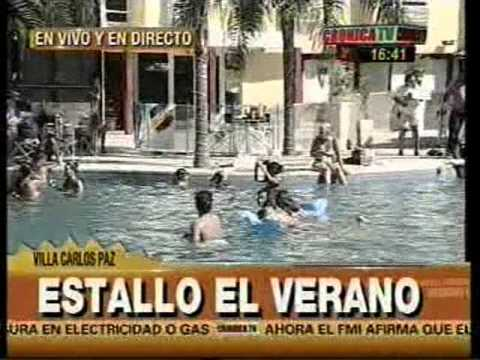
\includegraphics[width=0.9\textwidth]{../src/images/presentacion/estalloelverano.jpg}
        % \caption{} 
        \label{fig:estalloelverano}
        \end{figure}
    \end{column}
    \begin{column}{.30\textwidth}   
        \begin{figure}
        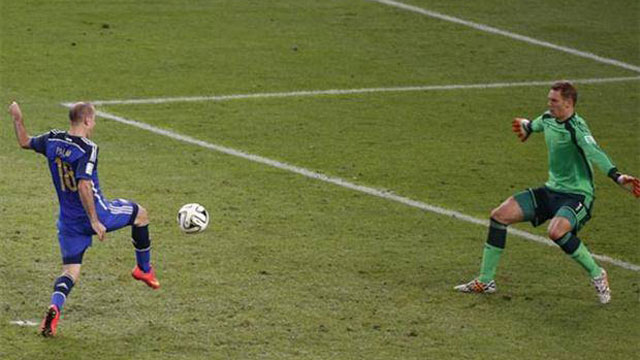
\includegraphics[width=0.9\textwidth]{../src/images/presentacion/eraporabajo.jpg}
        % \caption{} 
        \label{fig:eraporabajo}
        \end{figure} 
    \end{column}
    
    \end{columns}


  \begin{figure}
    \begin{columns}%
        \begin{column}{0.65\textwidth}%
            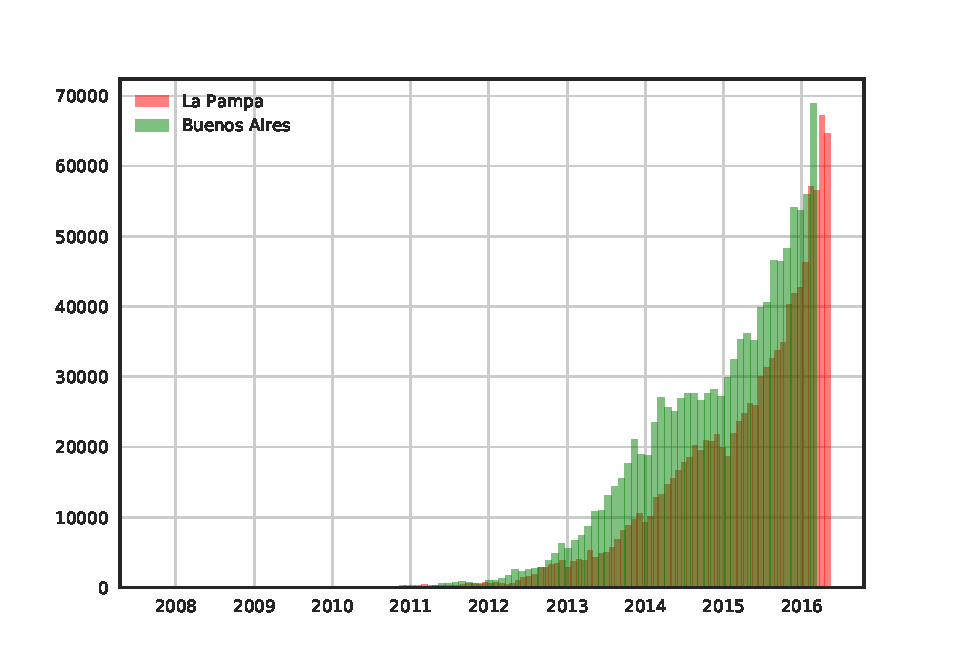
\includegraphics[width=.8\textwidth]{../src/images2/histTweetsProvincia1_sinFiltro.pdf}
        \end{column}%
        \begin{column}{0.33\textwidth}%
            \caption{Histograma de la cantidad de tuits que se hicieron por intervalo de tiempo en la provincias La Pampa y Buenos Aires.}
        \end{column}%
    \end{columns}
\end{figure}

\end{frame}

\begin{frame}[c]\frametitle{Balanceo de cantidad de tuits y de usuarios}
    
    \begin{table}
\centering
\scalebox{0.6}{
\begin{tabular}{|l|c|c|c|c|c|c|}
\hline
Provincia      & \#Palabras Distintas & \#Usuarios & \#Tuits & \#Total Palabras \\ \hline
Buenos Aires   & 191919       & 920          & 1125042    & 8974372  \\
Catamarca      & 173104       & 957          & 1057019    & 8161309   \\
Chaco          & 169476       & 964          & 976943     & 7605991   \\
Chubut         & 182592       & 954          & 1023373    & 8884745   \\
Córdoba        & 207307       & 987          & 1224266    & 10075932  \\
Corrientes     & 183292       & 939          & 1044951    & 8426940   \\
Entre Ríos     & 188679       & 969          & 1193693    & 9462986  \\
Formosa        & 169254       & 903          & 923352     & 7184382   \\
Jujuy          & 171064       & 971          & 678004     & 5951778   \\
La Pampa       & 186593       & 935          & 1085757    & 8996318  \\
La Rioja       & 186041       & 946          & 704044     & 6757277  \\
Mendoza        & 193708       & 945          & 1099717    & 9402399   \\
Misiones       & 168400       & 972          & 984218     & 7790197   \\
Neuquén        & 188038       & 927          & 1111201    & 9021449   \\
Río Negro      & 194383       & 965          & 1215361    & 9991831  \\
Salta          & 188402       & 884          & 830916     & 7506652   \\
San Juan       & 183546       & 926          & 1002322    & 8377792  \\
San Luis       & 164185       & 896          & 1006464    & 8327093  \\
Santa Cruz     & 174089       & 935          & 876621     & 7432923  \\
Santa Fe       & 201879       & 937          & 1019620    & 8862328  \\
S. del Estero       & 166540       & 887          & 944109     & 7355729  \\
T. del Fuego & 197273       & 964          & 976426     & 8559218   \\
Tucumán        & 195643       & 962          & 1093874    & 9238526 \\
  \hline
\end{tabular}}
\caption{Cantidades del conjunto de datos}
\label{tab:cantidades}

\end{table}


\end{frame}

\subsection{Tokenización y normalización}

\begin{frame}[c]\frametitle{¿Qué es una palabra?}
    \begin{block}{Tokenización}
    Palabra = secuencia de caracteres alfabéticos (letras)
    \begin{multicols}{2}
    \begin{itemize}
        \item \#estalloElVerano $\rightarrow$ \xmark
        \item \smiley{} \frownie{} $\rightarrow$ \xmark
        \item https://nic.ar/ $\rightarrow$ \xmark
        \item @BombitaDarin $\rightarrow$ \xmark
        \item siempr3 $\rightarrow$ \xmark
        \item siempre $\rightarrow$ \cmark
    \end{itemize}

    \end{multicols}
    % Decidimos ignorar estos términos ya que no tienen interés lingüístico y agregarían mucho ruido a los datos.
    \end{block}

    \begin{block}{Normalización}
    \begin{itemize}
        \item \textbf{Minúscula:} Casa,CaSA,casA $\rightarrow$ casa
        \item \textbf{Hasta 3 repeticiones:} jajaaaaaa $\rightarrow$ jajaaa
    \end{itemize}
    \end{block}

\end{frame}

\begin{frame}[c]\frametitle{Cantidades por provincia}
    \begin{table}[ht]
\centering
\begin{tabular}{|c|cccc|c|}
  \hline
Palabra &Prov.1& Prov.2 &$\cdots$ Prov.23& Totales \\
  \hline
  $w_1$& $N_{1,1}$& $N_{1,2}$ &$\cdots$
  $N_{1,23}$ & $\mathbf N(w_1)$\\
    $w_2$& $N_{2,1}$& $N_{2,2}$&$\cdots$
    $N_{2,23}$ & $\mathbf N(w_2)$\\
  $\cdot$& $\cdot$& $\cdot$ &$\cdots$
          $\cdot$ & $\cdot$\\$w_i$& $N_{i,1}$& $N_{i,2}$ &$\cdots$
      $N_{i,23}$ & $\mathbf N(w_i)$\\
    $\cdot$& $\cdot$& $\cdot$ &$\cdots$
          $\cdot$ & $\cdot$\\
            $\cdot$& $\cdot$& $\cdot$ &$\cdots$
                    $\cdot$ & $\cdot$\\  $\cdot$& $\cdot$& $\cdot$ &$\cdots$
                              $\cdot$ & $\cdot$\\
      \end{tabular}
\end{table}

\noindent donde $N_{i,j}$ representa la cantidad de veces que la palabra $w_i$ aparece en la provincia Prov.$j$, $j=1,\ldots, 23$. 
\begin{equation}
\mathbf N(w_i)=\sum_{j=1}^{23} N_{i,j}
\end{equation}

% \hyperlink{valoresContrastivos}{\beamerbutton{Volver}}

\end{frame}